%!TEX root = project.tex

\chapter*{About this project}
\paragraph{Abstract}
A dynamic web app that creates curated playlists based on multiple user's music preferences using Spotify. Built with React, Flask, Python, Node.js, Mocha, AWS and Mongo.

\paragraph{Authors}
\begin{flushleft}
	Eddie Eldridge
	
	Danielis Joniskis
	
	Keith Higgins 
	
	Three students from the Galway-Mayo Institute of Technology
\end{flushleft}



\chapter{Introduction}
The introduction should be about three to five pages long.
Make sure you use references~\cite{einstein}
\begin{flushleft}
	Context for the Project.
	
	
	Objectives of the Project.
	
	
	Is the reader 100 percent of what the project is all about 
\end{flushleft}


\chapter{Context}
The context of this project revolves around the use case of multiple people sitting together in a car or house and not being able to design on what music to play. One of the people can open the app and generate a play list that they can all enjoy instead of spending time on deciding what to play specifically.

The goal of our project was to develop a dynamic web application that creates curated playlists based on multiple user's music preferences using Spotify.

The project was completed over a 7-month period and this meant that the project environment didn’t change drastically.

\section{Project Reference}
https://github.com/WePickOrganization/WePick

\section{Objectives}
The project required several objectives to be accomplished in order to provide a solution that worked.
\begin{itemize}
	\item Set up a MongoDB database that will be used to store the user’s preferences along with the user’s email and password.
	\item Host the application in the cloud – using AWS. This must be done so the application can be accessed from any desktop.
	\item Set up a user interface using React, which will serve as the frontend for the application.
	\item Make use of Flask and Python to set up the backend for the application.
	\item Use the Spotify API to generate the playlist.
\end{itemize}

\section{Overview}
Each chapter of this minor dissertation gives different details on this group project.

The Methodology outlines the different options that were considered to design the solution. Project management and development methodologies are outlined here.

The Technology Review discusses in detail, the different technologies that were used throughout the project.

The System Design gives a rundown on each part of the system, the technologies used to build each part and how they work.

The System Evaluation section evaluates the project against the objective and proves robustness and performance of the project.

The Conclusion will be a reflection on the project.


\chapter{Methodology}
About one to two pages.
Describe the way you went about your project:
\begin{itemize}
\item Agile / incremental and iterative approach to development. Planning, meetings.
\item What about validation and testing? Junit or some other framework.
\item If team based, did you use GitHub during the development process.
\item Selection criteria for algorithms, languages, platforms and technolo-gies.
\end{itemize}
Check out the nice graphs in Figure \ref{tikz:graphs}, and the nice diagram in Figure \ref{tikz:mydiagram}.

\begin{figure}
  \centering
  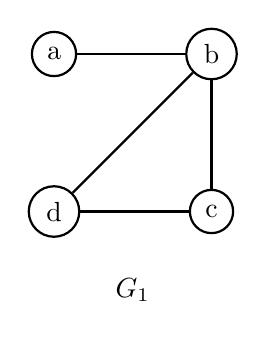
\begin{tikzpicture}
  \begin{scope}[every node/.style={circle,thick,draw}]
  \node (a) at (0,2) {a};
  \node (b) at (2,2) {b};
  \node (c) at (2,0) {c};
  \node (d) at (0,0) {d};
  \end{scope}
  \begin{scope}[every edge/.style={draw=black,thick}]
  \path (a) edge (b);
  \path (b) edge (c);
  \path (b) edge (d);
  \path (c) edge (d);
  \end{scope}
  \node () at (1,-1) {$G_1$};
  \end{tikzpicture}
  \hspace{1.5cm}
  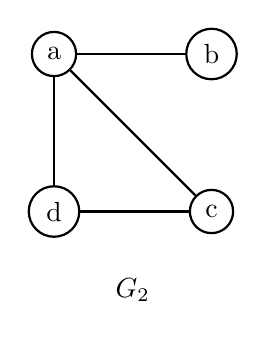
\begin{tikzpicture}
  \begin{scope}[every node/.style={circle,thick,draw}]
  \node (1) at (0,2) {a};
  \node (2) at (2,2) {b};
  \node (3) at (2,0) {c};
  \node (4) at (0,0) {d};
  \end{scope}
  \begin{scope}[every edge/.style={draw=black,thick}]
  \path (1) edge (2);
  \path (1) edge (3);
  \path (1) edge (4);
  \path (3) edge (4);
  \end{scope}
  \node () at (1,-1) {$G_2$};
  \end{tikzpicture}
  \caption{Nice pictures}
  \label{tikz:graphs}
\end{figure}


\begin{figure}
  \centering
  \begin{tikzpicture}[node distance=6cm]
  \node (a) [rect] {A Big Blue Block};
  \node (b) [oval, right of=a] {And His Oval Friend};
  \draw [line] (a) -- (b);
  \end{tikzpicture}
  \caption{Nice pictures}
  \label{tikz:graphs}
\end{figure}


\chapter{Technology Review}
About seven to ten pages.
\begin{itemize}
\item Describe each of the technologies you used at a conceptual level. Standards, Database Model (e.g. MongoDB, CouchDB), XMl, WSDL, JSON, JAXP.
\item Use references (IEEE format, e.g. [1]), Books, Papers, URLs (timestamp) – sources should be authoritative. 
\end{itemize}

\section{AWS}
Amazon Web Services offers reliable, scalable, and inexpensive cloud computing services.

\begin{minted}{xml}
<this>
  <looks lookswhat="good">
    Good
  </looks>
</this>
\end{minted}

\section{MongoDB}
MongoDB is an open-source, document database designed for ease of development and scaling. MongoDB stores data in JSON-like documents, which makes the database very flexible and scalable.\cite{w3schools}

\section{Flask}
Flask is a microframework for Python.

\section{Python}
Python is a programming language that lets you work more quickly and integrate your systems more effectively.

\section{Mocha}
Mocha is a JavaScript test framework running on Node.js. Mocha tests run serially, allowing for flexible and accurate reporting

\section{React}
React is a JavaScript library for building user interfaces. React is developed by Facebook. It is a tool for building UI components. React uses Babel to convert JSX (JavaScript XML) into JavaScript. Babel is a JavaScript compiler that can translate markup or programming languages into JavaScript. With Babel, you can use the newest features of JavaScript (ES6 - ECMAScript 2015). \cite{w3schools}

\chapter{System Design}
We looked at different architectures for our web application and decided to use 3-tier architecture. In doing this we were able to separate the work between the group, purposely playing to each team members strengths. Utilizing a 3-tier architecture allowed us to comfortably work on one tier without impacting the other tiers directly. It proved especially useful when a update came out for the technology at a given layer, we were able to update that layer independently without trouble.


We opted to utilise a 3-tier architecture consisting of the following components:

\begin{center}    
	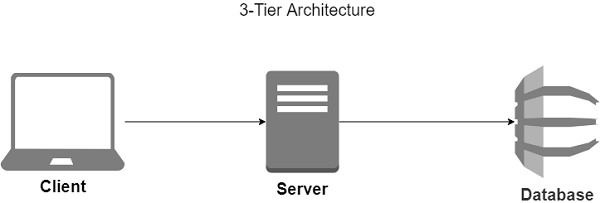
\includegraphics{img/3tier.png}
\end{center}

\subsection{React frontend (Client)}
The React front-end is what you see at the Presentation layer. This is what the user is interacting with on their own PC. On this tier input is received, and output is displayed.
We used ReactJS for the front-end as there is good support for it. A great thing about React is that you can create reusable UI components. React is good for its simplicity. It makes use of JSX syntax which allows you to produce React elements more intuitively, but still also allows you to write in plain Javascript.


The React front end consists mainly of index.jsx and several separate component classes. The index page acts an entry point and is the outermost component class in the React application. The index page handles the user logging in by passing in the email from the LoginForm component. Once the details are verified, the user is redirected to the Create page which contains the ArtistEnter component. The index page handles the user logging out by clearing the logged in state and redirecting back to the Home page. 
The index page is where the React components are rendered visually. The Home page components displayed consist of the NavBar, Carousel, Home, GenerateButton, and StickyFooter. 

There is also an app form which consists of the ArtistEnter, Logout, RegisterForm, Auth, LoginForm and Prefs.

These components are then styled with multiple CSS files.


The LoginForm component takes in the user’s email and password. Once the user clicks on the submit button. An Axios GET request is performed. Sent to the Flask servers createUser route.

The Logout component simply clears any state held by its parent component and then redirects to the Home page.

The Home component acts as the component between the NavBar, Carousel and StickyFooter components. The Home component is where the GenerateButton component is rendered.

The NavBar component contains the navigation bar that is always rendered in the application. The user can follow the links on the NavBar to the Home, Create and Profile pages respectively.

The Carousel component is used to render an image carousel on the Home page. The carousel cycles through 7 different images and is a style choice which gives a more professional look to the application.

The Auth component handles authorization.

The RegisterForm component renders the form which is displayed to the user when they are registering a new account in the application. It takes in the user’s name, email and password. On submit the user’s information is routed to auth.

The ArtistEnter component contains the form which allows the user to generate a play list based on their preferences. Once the user has logged in successfully, they can enter four different artists of their choosing and their email address. The user can then generate a playlist by submitting the form.

The Prefs

\subsection{Python backend (Server)}
The python backend is what is present at the Application layer. This is the server which is made using flask and python. On this tier the logic is processed, and calculations are made.
SpotipyAPI.py is where the playlist generation is handled behind the front-end. When an artist is searched, a lot of information about the artist is returned i.e. Hometown etc.
The JSON data that is returned is where their artist ID is stored. This in-turn allows us to grab that artist ID and use it in generating the playlist. 

We make use of OAuth 2.0; this is the industry standard protocol for authorization. We use OAuth2 to authenticate the user through Spotify. When the user is trying to login to their account on our application, they are in turn brought to a login dialogue through their Spotify account. Once they have logged into Spotify they are authorized and can continue with our application. 

\begin{center}    
	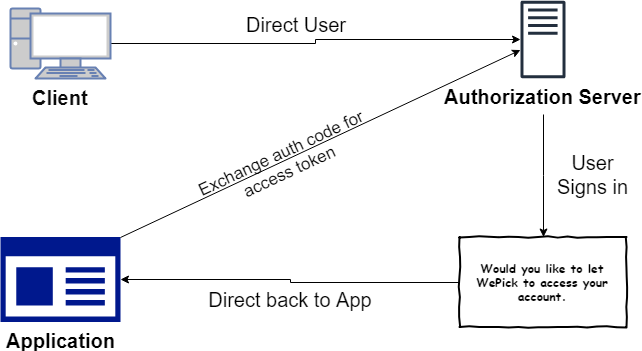
\includegraphics{img/auth.png}
\end{center}
The user starts out by going to the application. The application then sends the user to the authorization server. The user logs in here and the authorization server sends the user back to the application. The application then makes a POST request to the authorization server to get an access token.

\subsection{MongoDB (database)}
The MongoDB is what is at the Data layer. On this tier data is stored and managed. Once the database was set up, we wrote DatabaseConnector.py. We loaded in the IP address and password for the database from a config file found locally on the machine. Once the database was created, we could view the collection of users in the database. We made use of functions to add, show and delete users. We also wrote a function which could be used to show a user and their favourite artist from the database.

\chapter{System Evaluation}
In this chapter, we will discuss many aspects of the software. We will break the evaluation down into 4 headings.
\begin{itemize}
  \item Robustness - How well the software can deal with problems, it's ability to handle change etc.
  \item Performance - Space and time complexity of the software, responsiveness etc.
  \item Security - How vulnerable is the application to attacks and security risks?
  \item Overall evaluation - Where the project succeeded/failed, limitations in our approach and technologies etc.
  \end{itemize}

  \subsection{Robustness}
  Robustness in regards to software can be defined as the ability of the software to cope with errors during execution and cope with erroneous input. Measuring the robustness of a system is difficult 
  as no system can be considered completely robust. However, there are certain methodologies and practices we can implement to increase the robustness of a system. {\textit{Behdis Eslamnour and Shoukat Ali}} discuss these metrics in their paper entitled {\textit{Measuring robustness of computing systems}}\cite{SoftwareRobustness}
  Some of these proposed metrics include
    \newline
    \begin{itemize}
      \item Error Handling/Error Catching
      \item Time between failures and time between recovery
    \end{itemize}

    \subsection{Error Handling}
    Error handling refers to how a system handles errors should they occur. This can be as simple as logging the error in the console to rolling back the system to a previous stable release.
    It is a vital aspect for any system from both the perspective of the user and developer. As a developer, implementing proper error handling and catching is an important aspect of development
    as it enables the developer to work more effectively and efficiently as less time is spent fixing and locating the cause of bugs if proper error handling is done pre-emptively.

    For the user, it's vital that error handling is done correctly as incorrect error handling can have a significant impact on the end-users experience of the system/software. For example, if a user
    attempts to login to a system and their login details are incorrect, a meaningful way of handling this error would be to notify the user that their login details are incorrect. If this is not done, 
    the end user won't understand what's happening and why they can't use the system and as a result of this will become frustrated/unhappy with the service. As such it's important to make sure any critical
    problems such as this are caught and handled in an appropriate manner. However, it's also important to remember that complete robustness can not be achieved and as such one must try and figure out the 
    most important and likely errors to handle. When making these decisions, one can consider many factors when deciding what errors to handle such as the risk of not handling the error (application crashing, unexpected behaviour, potential security risk, loss of data etc.)
    , how much time will be required to handle the error and the likelihood of the error occuring. However, as mentioned above complete robustness can not be achieved as to even consider the above factors,
    one must have the foresight to see that the error will occur in the firstplace.

    Below I will discuss some error handling that occured in our project and how it contributed to the overall robustness of the system.
    
    \textbf{Example 1 - Login/Register} 
    In the image below we can see how error handling and error catching can produce meaningful output and guide the user through login/register scenario of our application

    ---- user login diagram here ----

    \textbf{Example 2 - Authentication with Spotify}
    In the image below we can see how error handling and error catching can produce meaningful output and guide the user through authenticating our applicatin with Spotify.

    --- authentication diagram here ----


    The above error handling was done on both the server and client-side of the application. Both Python, MongoDB and Pythn provide useful tools for error handling/catching.
    Some examples include \textit{Error boundaries} in React, \textit{Try/Catch/Raise statements} and \textit{Schema validation} in MongoDB.

    \begin{itemize}
      \item Error Boundaries - Error boundaries are React components that catch JavaScript errors anywhere in their child component tree, log those errors, and display a fallback UI instead of the component tree that crashed.
      \item Try/Catch/Raise statemetns - These commonly found in most programming languages and Python is no exception. We used these to catch certain errors such as HTTPErrors, null value errors, MongoDB errors and many others.
      \item Schema Validation - To ensure the data being passed into the Mongo database was in the correct format, we used a JSON Schema to validate our inputs against before passing it to Mongo. In the below example, we can see that for a user 
      to be validated correctly, the minimum required properties are an email and password. This ensures that user's cant create accounts without these two required properties.
      \begin{minted}{JSON}
      user_schema = {
        "type": "object",
        "properties": {
            "name": {
                "type": "string",
            },
            "email": {
                "type": "string",
                "format": "email"
            },
            "password": {
                "type": "string",
            },
            "spotifyUsername": {
                "type": "string",
            },
          
        },
        "required": ["email", "password"],
        "additionalProperties": False
      }
      \end{minted}
      
    \end{itemize}

    \subsection{Time between failures and time between recovery}
    Time between failures and time between recovery are too very useful metrics in determining the robustness of a system. Systems that have a short mean time between failures and mean time between recovery
    either have excellent error handling or are designed in such a way that errors do not occur frequently. A good way of measuring this could be 
    the downtime of your application over the course of a year. For example, on average, the top 50 e-commerce websites experienced 99.03\% uptime. Over a year, 99.03\% uptime would result in 3 days 15 hours and 39 minutes of downtime. 32 of
    these websites experienced 99.99\% uptime. 9 out of 10 of users encountering a website that is not up will choose to use a competitors website \cite{WebsiteDowntimeStats}. From these statistics, we can see that time between failures anre time between recovery are extremely important aspects to 
    any system/application. As such, they can be very helpful metrics when trying to measure the robustness of an application. 

    In regards to WePick's failure and recovery time, since the project was hosted on AWS' Elastic Beanstalk, there have been little to no outages as due 
    to the continous integration solution integrated upon deployment, it was not possible for broken code to be deployed as any code proposed to be deployed had 
    to first pass tests that were outlined by Travis CI and any problems that did arrive were dealt with quickly as Travis instantly notified us of any problems which we were 
    able to fix quickly and promptly.

    \subsection{Performance}
    When planning and designing the project, one of our main aim's was that we wanted the project to perform operations and tasks quickly as well as being responsive to user input. Taking these considerations into account, we choose
    Python and MongoDB for our backend as they are generally considered lightweight and easier to handle performance than say something like Java. We chose React for the front-end of the application as React is well known for it's performance and
    responsiveness. This generally comes from the fact that React applications usually implement a single page design. React works by creating multiple components that can be re-used multiple times in the application. For example, in our 
    application, instead of creating multiple pages with the same code (Navbar, Footer, Forms etc.), we can create seperate components for each of these items and only re-render what is required. So if the user needs a different form only that form will
    be re-rendered and the Navbar and Footer don't need to be re-rendered This choice of technology helped us achieve our overall goal in regards to perfromance and I think it was a good choice.

    Our choice of MongoDB as a database was also important to the overall perfromance of our application as MongoDB is considered much faster than SQL and other relational databases in certain scenarios. This is because of it's non-relational, no-SQL way of storing data.
    Instead of storing data in rows, columns and tables, Mongo works by using a document style architecture. These documents are structured similarly to a JSON document and as such are easy to extract data from and manipulate without navigating through 
    large sets of data like you would in a traditional SQL database. Generally, this performance increase can be seen most when you start to scale up the size of your database. For our application, it was important to be able to access user's favorite artists
    quickly so that they didn't have to wait a long time to generate a playlist.  

    \begin{center}    
      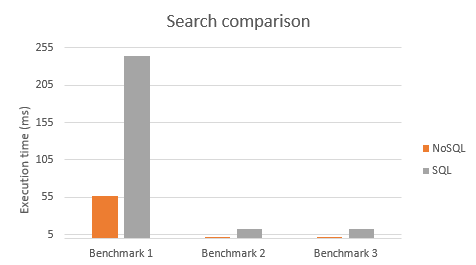
\includegraphics{img/SQLvsNOSQL.png}
    \end{center}

    From the above graph, we can see that when performing a search in the database, NoSQL databases like Mongo are considerably faster than a traditional SQL database /cite{SQLvsNOSQL}

    \subsection{Security}
    Securit was an important factor for us to consider when designing and creating the application as we had all experienced problems with group projects in the previous year. For example, many students dealt with problems where database tables were wiped and/or hijacked and held ransom
    to the owners. As such, we did not want to deal with such problems and thought it would be a good oppurtunity for us all to learn a bit more about how one goes about securing an application in a real world context. We also wanted user's information to be secure and not easily accessible by anyone.
    
    To ensure our RESTful routes were not accessible to anyone, we implemented JWT Tokens into our application. A JWT Token or JSON Web Token is an open-standard that defines a way for securely transmitting and verifiying information between systems.
    JWT's are signed using a secret key or a public/private key using RSA encryption.
    
    The way this ends up working in the application is as follows. When the user successfully logs in, a JSON Web Token is generated and each subsequent request
    made by the user will include that web token. Setting up the system in this way means that to perform a HTTP request on one of our many RESTFul routes, the user first has to 
    verify that they are an authenicated user. This prevents from people performing actions on routes that they should not have access to. 

    A traditional JSON Web Token consists of a Header, Payload and Signature in the following format 
    
    \begin{center}    
      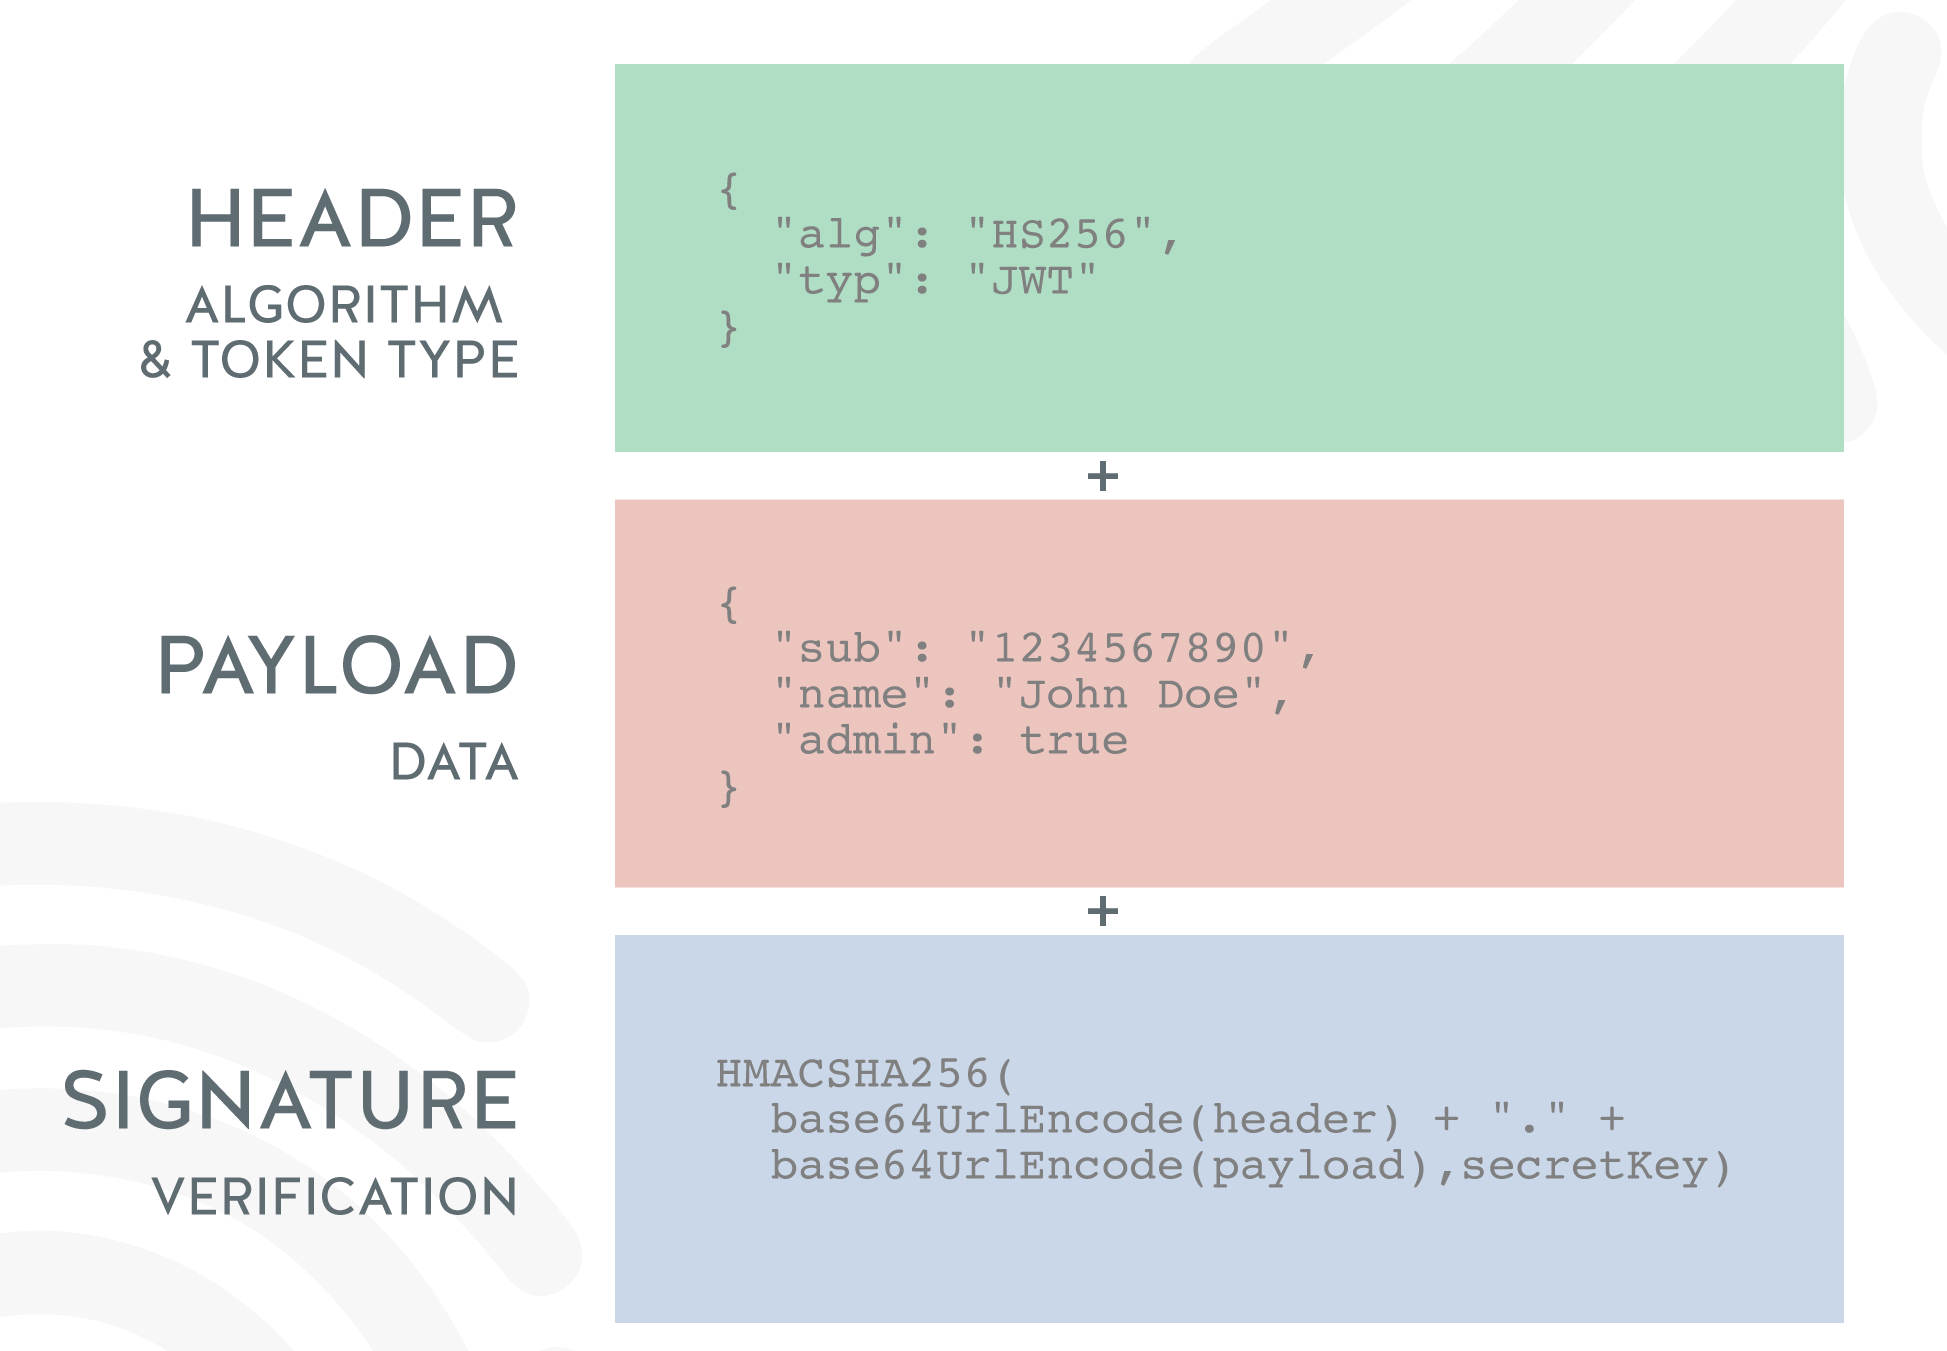
\includegraphics{img/JWTTokens.png}
    \end{center}

    \begin{minted}{JSON}
      header.payload.signature
    \end{minted}

    The header details what type of token is being sent and the algorthim used to generate the token.
    The payload contains the information about the person sending the token and what they would like to do.
    The signature is essentially an your header and payload encrypted and is used to verify the payload wasn't altered during transit as well as verifying the sender is who they say they are.
    
    An example token can be seen below

    \begin{center}    
      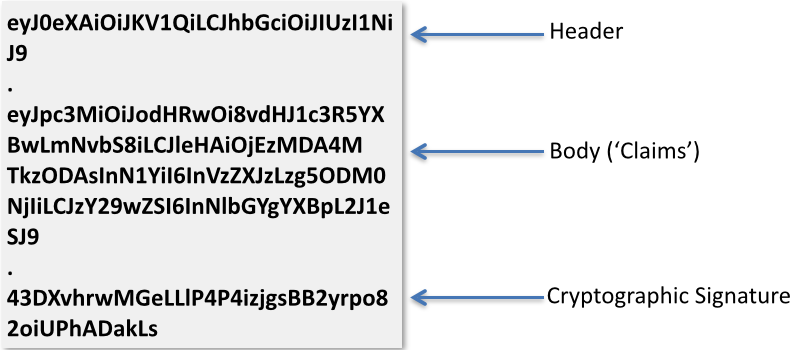
\includegraphics{img/JWTTokenHASH.png}
    \end{center}

    To implement this technology in our application, we used Flask-JWT, a simple Python library that provides JWT Support for Flask applications.
    A simple example of how this technology was implemented can be seen below.

    \begin{center}    
      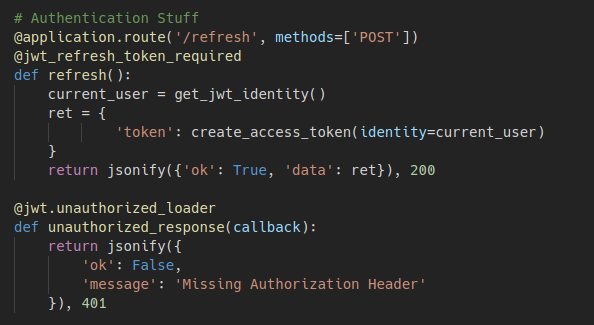
\includegraphics{img/JWTExample.png}
    \end{center}

    As well as ensuring API calls were authenicated, we also made sure that our database and user information was secure. A secure admin account was created on the database, requring a password to perform any actions in the databse.
    This way, no operations could be performed on the database without knowing both the IP address of the server the database was hosted on and the password required to gain access. These two important pieces of information were known only to us and 
    weren't available anywhere else. 

    We also made sure that any important user information such as passwords were encrypted before being entered into the databse.
    For this, we used another Python library for Flask entitiled Flask-Bycrypt. Using this library, we can generate a hash of the user's password and store this in the database instead of storing their password in plaintext. Then, when checking if 
    the user's login details are correct, we compare the generated hash of the passwords instead of the actual passwords themselves. This enables a secure login scenario and prevents passwords being revelead to anyone.

    To improve overall security, we also chose to host our application on a different instance than our database. This meant that if one were to be compromised in any way, it would prevent the other in turn being compromised.

    \subsection{Improving Security}
    \subsubsection{HTTP/HTTPS}
    One shortcoming of our project is the lack of a secure Hyper Text Transfer Protocol (HTTPS). HTTP can be described by Mozilla's standards /cite{HTTPviaMozilla} as an application-layer protocol 
    for transmitting data and documents. It was originally designed for communication between web browsers and web servers but it has since exceeded it's original purpose. It follows a client/server model. The client makes a 
    request to establish a connection and waits for a response from the server. Despite this however, it is a /bf{stateless} protocol. This means that once communication between server and client, the server forgets all information regarding
    the communication. It can be used on any reliable transfer layer such as TCP/IP or UDP.

    The difference between HTTPS and HTTP is that HTTPS is considered 'secure' where HTTP is not. Essentially, the difference between the two can be illustrated cleary in the following diagram.

    \begin{center}    
      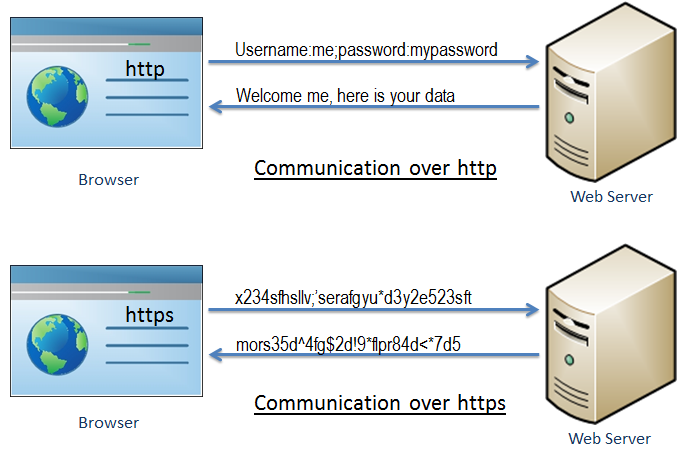
\includegraphics{img/HTTPS.png}
    \end{center}

    In standard HTTP, the information is transmitted in hypertext format whereas with HTTPS, the information is first encrypted before sending the information.
    The issue with standard HTTP is that the data is transmitted in plaintext. This means that anyone who can 'see' the data or is monitoring the network can potentially intercept this data and/or modify it before being passed on to the server. This can 
    lead to serious security issues. This could be potentially devestating to an application/system that relies on sensitive data such as passwords or bank/card details.

    HTTPS guarantees that even if the message is intercepted, it would be of no value as it is encrypted. HTTPS provides these guarantees using a security standard known as SSL or Secure-Socket Layer.
    SSL is a standard for establishing an encryped link between a client and server. To first use SSL, one must aquire an SSL certificate. These certificates are small files that bind a domain name/IP address/hostname to an organizational identity and location.

    \subsubsection{But who exactly has the authority to issue these certificates and how can we trust them?}
    To issue SSL certificates and guarantee their authenticity, one must become a Certificate Authority. 
    This title is usually limited to private companies and governments that have proven that the certificates they issue are secure. The more secure certificates they authorize, the more certificates they are able to distribute. 
    This means that when aquiring an SSL certificate, you can guarantee it's authenticity. A certified certificate should contain your domain name, company name, address, city, state, country. It also contains an expiration date upon which the certificate must be renewed as well as the Certificate Authority that issued the certificate in the first place.
    All these factors provide some kind of accountability in regards to the certificate if something were to go wrong. Expiring certificates is a common occurence, even for large companies. According to GlobalSign /cite{GlobalSign}, between just October 2017 and February 2018, large organizations such as LinkedIn, PokemonGO the British Conservative Party and astonglishly The White House 
    have all let their SSL certificates expire. Any users arriving on these websites would have been instantly greeted with a warning that these websites are not secure and sensitive information could have possibly been leaked in the process. For something like a goverment website, this kind of behaviour is a perfect example of why we have SSL and HTTPS in the first place and why it's vital that these systems are maintained and updated.

    \subsubsection{How does SSL work?}
    Let's use a traditional client/server architecture as our example. The browser/client connects to the server secured with SSL. The server will then prompt the client to identify itself.
    The server then sends a copy of it's SSL certificate. These certificate is then verified by the client. If verification is successful and the client is comfortable sending messages, it sends a response to the server which consists of a digitally signed acknowledgement which initiates an SSL encryped session.
    Any data exchanged between these two parties is now sent over the Secure-Socket Layer established by the client/server.


    \subsubsection{Benefits of SSL/HTTPS}
    We can describe the overall benefits of SSL/HTTPS as the following

    \begin{itemize}
      \item Utilize HTTPs, which elicits a stronger Google ranking.
      \item Create safer experiences for your customers.
      \item Build customer trust and improve conversions.
      \item Protect both customer and internal data.
      \item Encrypt browser-to-server and server-to-server communication.
      \item Increase security of your mobile and cloud apps.
    \end{itemize}

    \subsubsection{Why didn't we implement SSL/HTTPS?}
    Due to the nature of aquiring an SSL certificate, one usually has to purchase a certificate and pay a yearly fee for using it. We made a decision based on the information stored by our application and by factoring in the cost, decided that we didn't think it would be critical if HTTPS wasn't implemented.
    We understand it makes our application insecure, but we also understand why it makes it insecure and how this could be dealt with appropriately in future projects.


\chapter{Conclusion}
About three pages.

\subsection{Original Idea vs. Actual Implementation}
Our original idea/plan for this project was to create an application that created curated playlists based off multiple user's music preferences. This was our original idea before we had chosen any technologies or done any kind of design. Limiting the scope to this simple statement, I feel like we achieved our original goal that we set out in late September.
Up to 6 user's can go on our website, create an account, enter their music preferences and create a curated playlist of music based on their and their friends preferred music. We also wanted the website to be simple and intuitive to use without the user feeling overwhelmed or confused as the original purpose of the program was simple and as such the website should be simple to use.
We focused heavily on this as we all felt like that websites can be extremely overbearing and complicacted when sometimes the user just wants to perfrom a simple task and having to go through hoops to perform this simple task can be extremely frustrating.

\subsection{Learning Outcomes}
\subsection{Shortcomings/Oppurtunities}
\subsection{Closing Statement}
\subsection{Acknowledgements}

\begin{itemize}
\item Briefly summarise your context and ob-jectives (a few lines).
\item Highlight your findings from the evalua-tion section / chapter and any opportuni-ties identified.
\end{itemize}

